\documentclass[a4paper, 12pt]{extarticle}
\usepackage[dvipsnames]{xcolor}
\usepackage[top=70pt,bottom=70pt,left=48pt,right=46pt]{geometry}
\definecolor{header}{RGB}{252, 171, 16}
\definecolor{defenition}{RGB}{248, 51, 60}
\definecolor{main_title}{RGB}{43, 158, 179}
\definecolor{sub_header}{RGB}{68, 175, 105}
\usepackage[english, russian]{babel}
\usepackage[utf8]{inputenc}
\usepackage{amsmath}
\usepackage[most]{tcolorbox}
\usepackage{listings}
\usepackage{graphicx}
\usepackage{amsmath}
\usepackage{lettrine}
\usepackage{wrapfig}
\title{\textcolor{main_title}{Инжекционные полупроводниковые лазеры}}
\author{Шмаков Владимир Евгеньевич - ФФКЭ гр. Б04-103}


\newtcolorbox{fequation}[1][]{ams equation*,size=small,#1}








\begin{document}
\maketitle



\section*{\textcolor{header}{Цель работы}}
\begin{itemize}
    \item Снять выходные характеристики светодиода и полупроводникового лазера
    \item Снять спектры излучения светодиодов
\end{itemize}
\section*{\textcolor{header}{Теоретические сведения}}

\lettrine{\textcolor{defenition}{П}}{\textcolor{defenition}{олупроводниковый инжекционный лазер}} состоит из активной области, расположенной между двумя полупроводниковыми слоями с разными типами проводимости, где за счет электрического тока происходит инжекция носителей и их рекомбинация, которая сопровождается излучением  света. Роль резонатора в ПИЛ выполняют скошенные грани кристалла.

Необходимым условием генерации является превышение коэффициента усиления над потерями в резонаторе. Пороговый ток накачки, необходимый для генерации ПИЛ задаётся формулой \ref{eq:thr}.
\begin{equation}
    j_{\text{порог}} = j_0 + \frac{\alpha}{\beta} + \frac{1}{2 \beta L} \operatorname{ln}\left( \frac{1}{R_1 R_2}\right)
    \label{eq:thr}
\end{equation}
\begin{itemize}
    \item $j_0$ - плотность тока инверсии
    \item $\alpha$ - коэффициент поглощения
    \item $L$ - расстояние между скошенными гранями кристалла
    \item $\beta$ - коэффициент усиления по току
    \item $R_1$, $R_2$ - коэффициенты отражения граней
\end{itemize}





\section*{\textcolor{header}{Методика}}

\subsection*{\textcolor{sub_header}{Оборудование}}
\begin{itemize}
    \item Фотоприёмник
    \item Монохроматор
    \item Блок питания
    \item Амперметры и вольтметры
    \item ПИЛ и набор светодиодов
\end{itemize}

\subsection*{\textcolor{sub_header}{Экспериментальная установка}}


\begin{figure}[htbp]
    \centering
    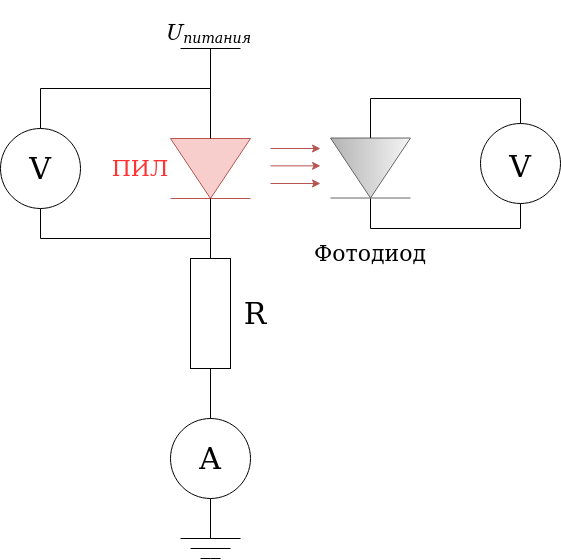
\includegraphics[width = 0.5\textwidth]{scheme.png}
    \caption{Схема экспериментальной установки}
    \label{fig:setup}
\end{figure}

Схема экспериментальной установки изображена на рисунке \ref{fig:setup}. Регулируя напряжение питания $U_{\text{питания}}$ изменяем силу тока накачки. Напряжение на исследуемом ПИЛ фиксируется при помощи вольтметра. Сила тока, текущая через ПИЛ фиксируется при помощи амперметра. Для регистрации интенсивности излучения ПИЛ используется фотодиод, напряжение на котором пропорционально интенсивности падающего света.

Для регистрации спектра исследуемого образца в оптическую схему добавляется монохроматор. Вращая ручку монохроматора регистрируем интенсивности на различных длинах волн.

\section*{\textcolor{header}{Обработка экспериментальных данных}}

\subsection*{\textcolor{sub_header}{Выходные характеристики светодиода}}

\begin{figure}[htbp]
    \centering
    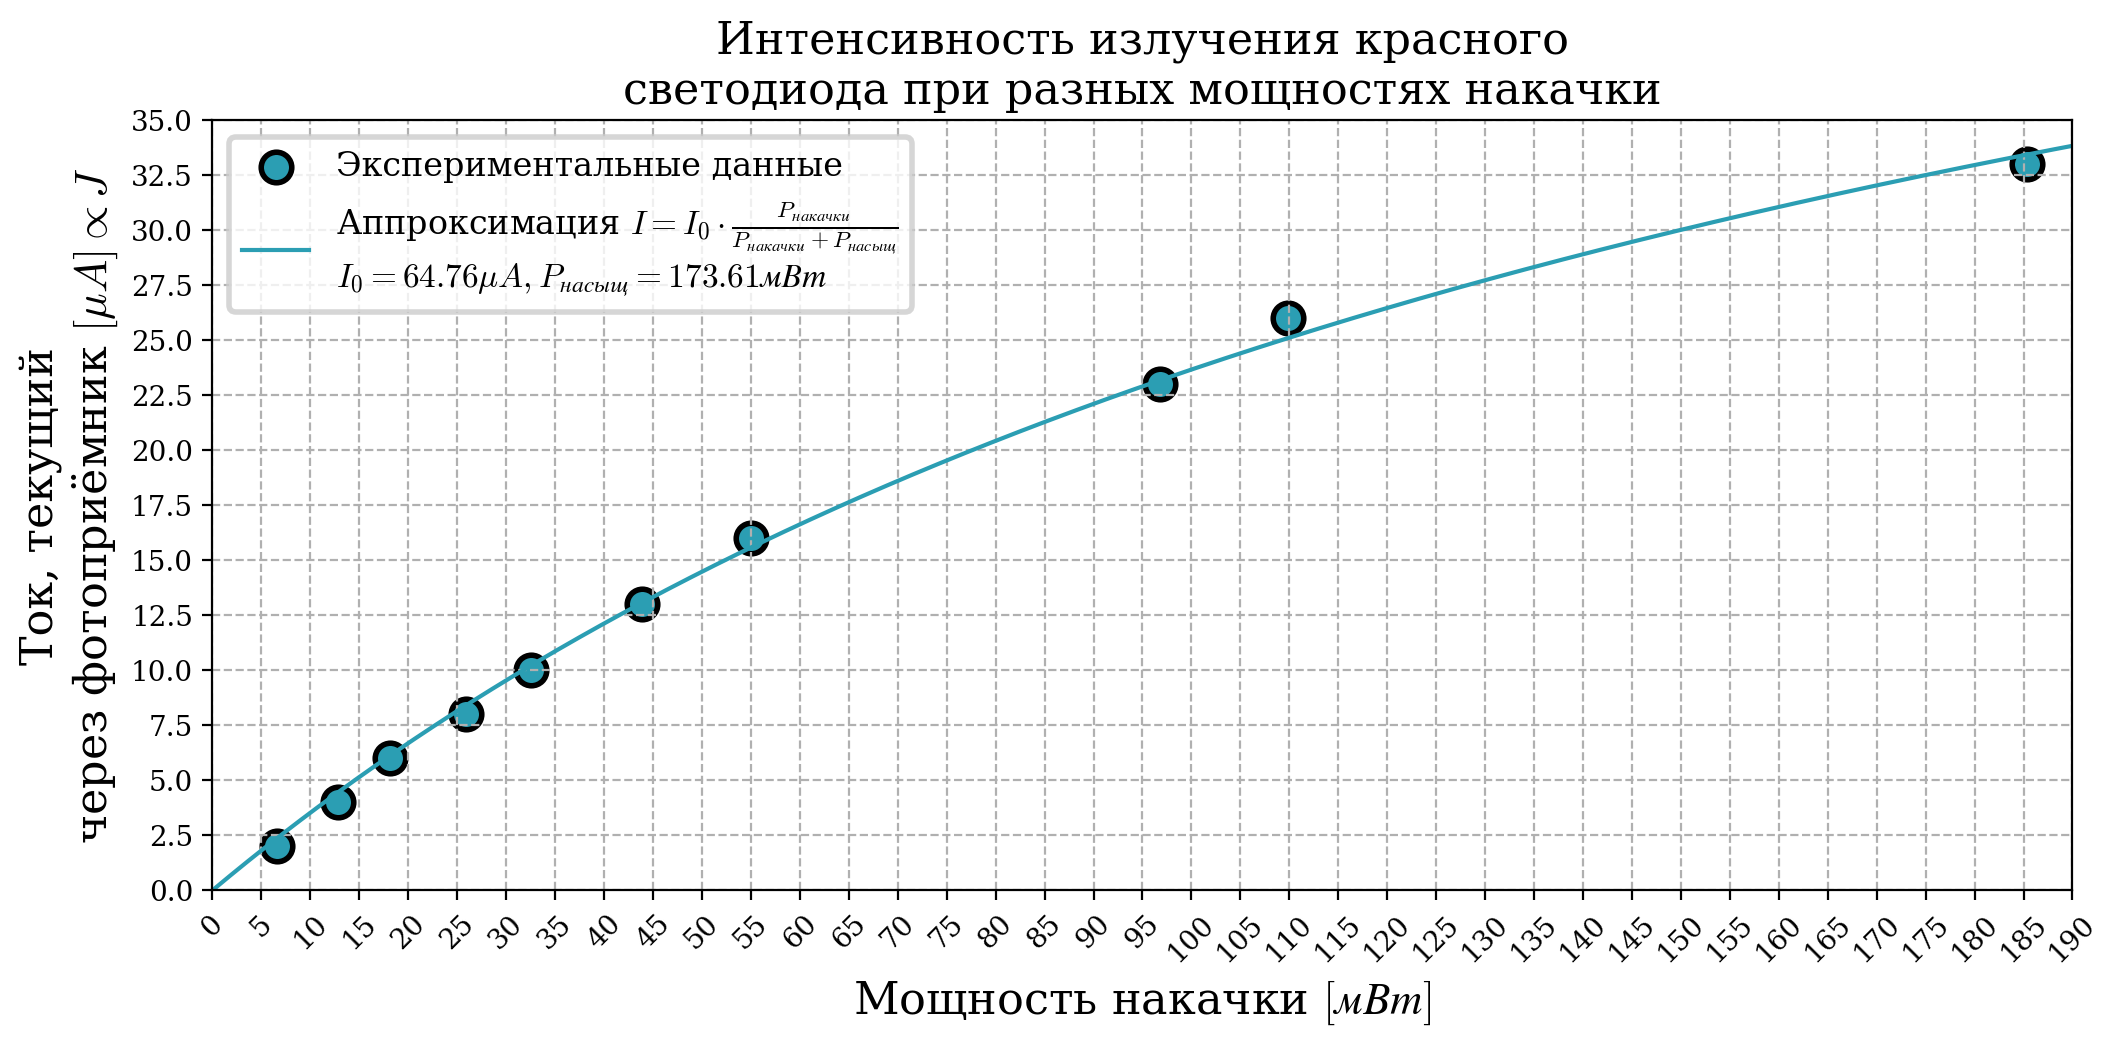
\includegraphics[width = 0.8\textwidth]{red_vc.png}
    \caption{Выходная характеристика красного светодиода}
    \label{fig:red_vc}
\end{figure}

Выходная характеристика красного светодиода изображена на рисунке \ref{fig:red_vc}. 
Как видно, с ростом мощности накачки растёт интенсивность излучения светодиода. При низках токах накачки число носителей заряда, попадающих в активную область, пропорционально силе тока --  интенсивность линейно зависит от мощности накачки. При высоких токах активная область перенасыщается носителями и повышение мощности накачки практически не приводит к увеличению интенсивности.


Аппроксимируем экспериментальные данные по формуле \ref{eq:vc}, и найдём мощность при которой светодиод входит в насыщение.

\begin{equation}
    I = I_0 \frac{P_{\text{накачки}}}{P_{\text{накачки}} + P_{\text{насыщения}}}
    \label{eq:vc}
\end{equation}

Результат аппроксимации изображен на рисунке  \ref{eq:vc}. <<Мощность насыщения>> оказалась равной $P_{\text{насыщения}} \sim 175 \text{мВт}$.



\subsection*{\textcolor{sub_header}{Выходные характеристики полупроводникового лазера}}



\begin{figure}[htbp]
    \centering
    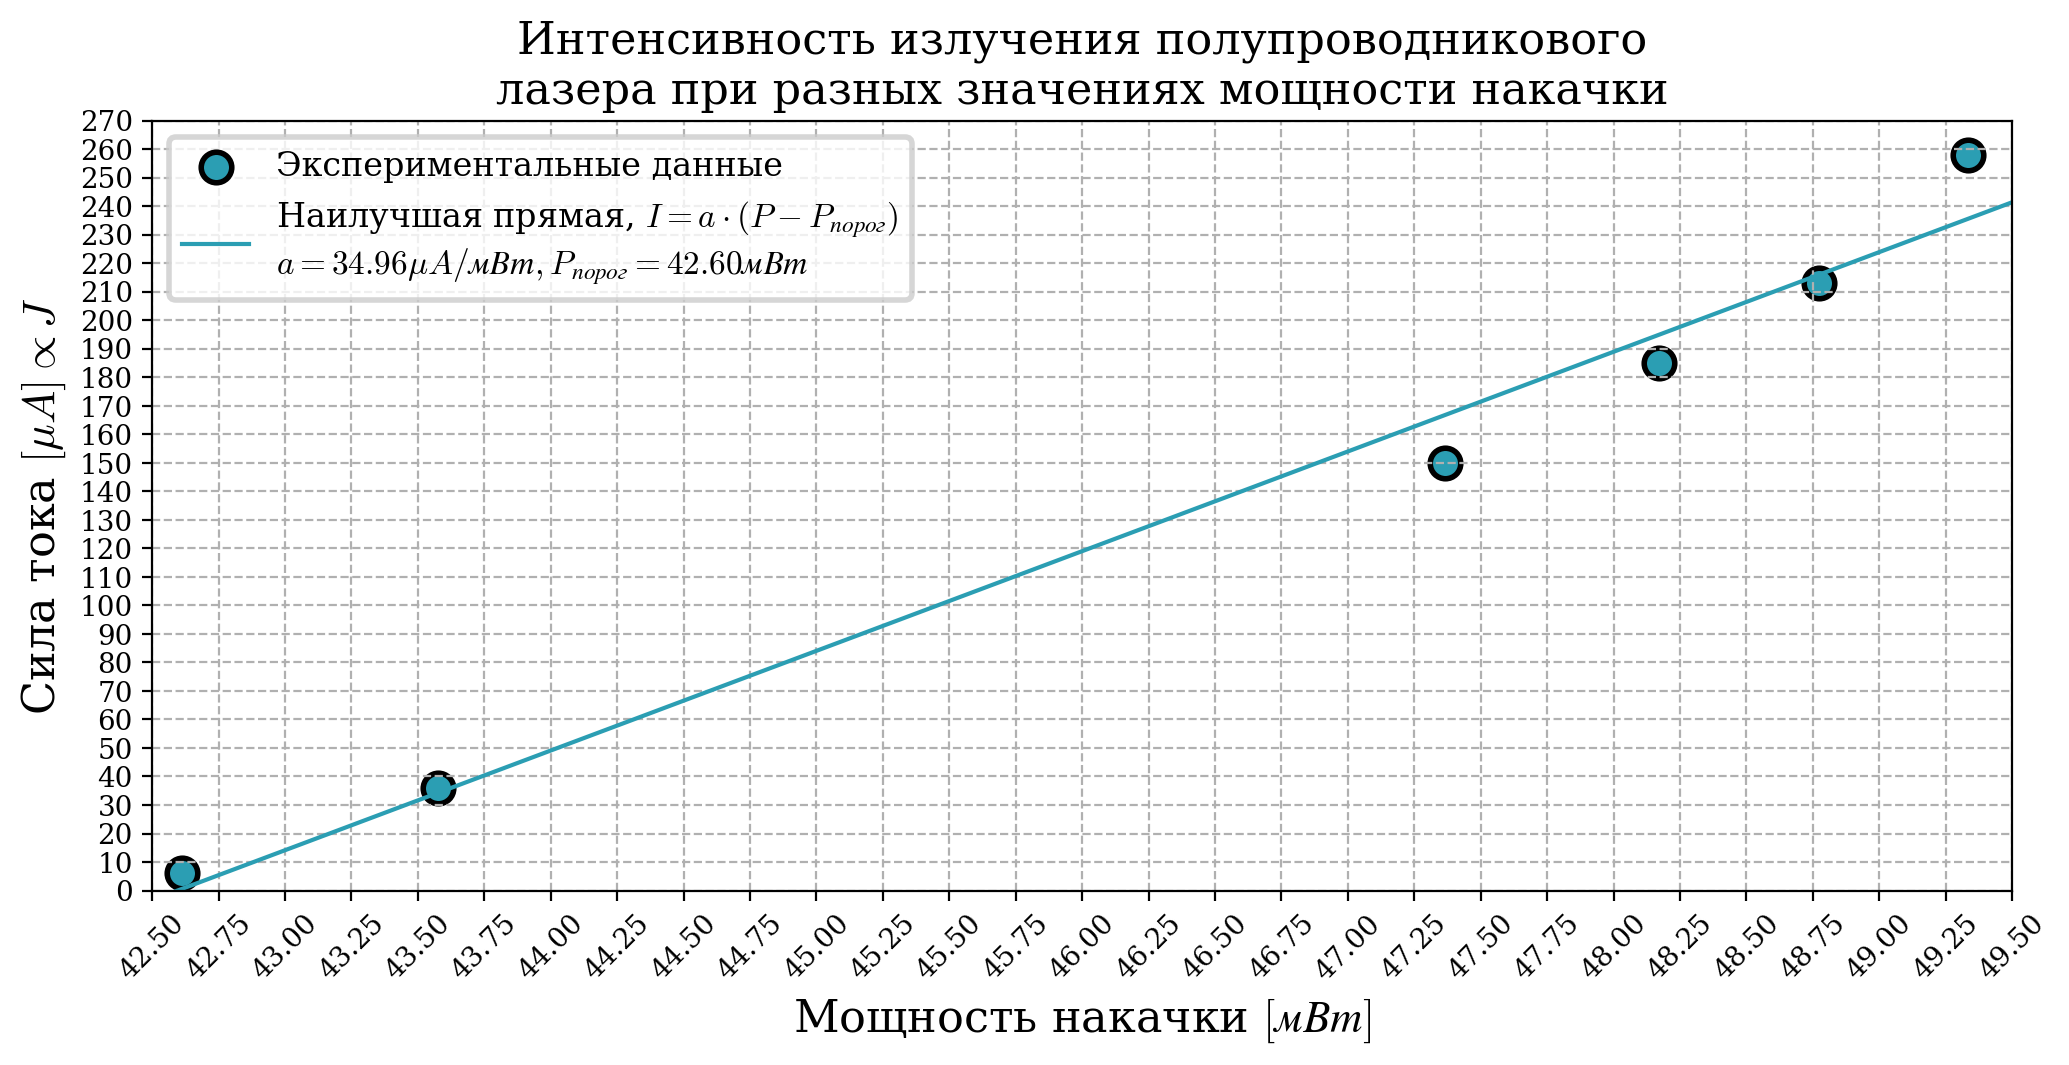
\includegraphics[width = 0.85\textwidth]{lazer.png}
    \caption{Выходная характеристика полупроводникового лазера}
    \label{fig:lazer}
\end{figure}

В отличие от светодиода, полупроводниковый лазер начинает излучать только в том случае, когда мощность накачки превышает некоторую пороговую величину. На рисунке \ref{fig:lazer} изображена линейная часть выходной характеристики полупроводникового инжекционного лазера. Найдём пороговую мощность накачки, для этого аппроксимируем экспериментальные данные по формуле \ref{eq:porog}.
\begin{equation}
    I = \alpha (P - P_{\text{порог}}) 
    \label{eq:porog}
\end{equation}

В результате аппроксимации получили что пересечение наилучшей прямой с осью $x$ равно $P_{\text{порог}} \sim 40 \text{мВт}$.

\newpage
\subsection*{\textcolor{sub_header}{Спектральные характеристики излучения синего светодиода}}
 

Экспериментально полученные спектры излучения различных светодиодов могут быть найдены в таблицах(4 - 6).
\begin{figure}[htbp]
    \centering
    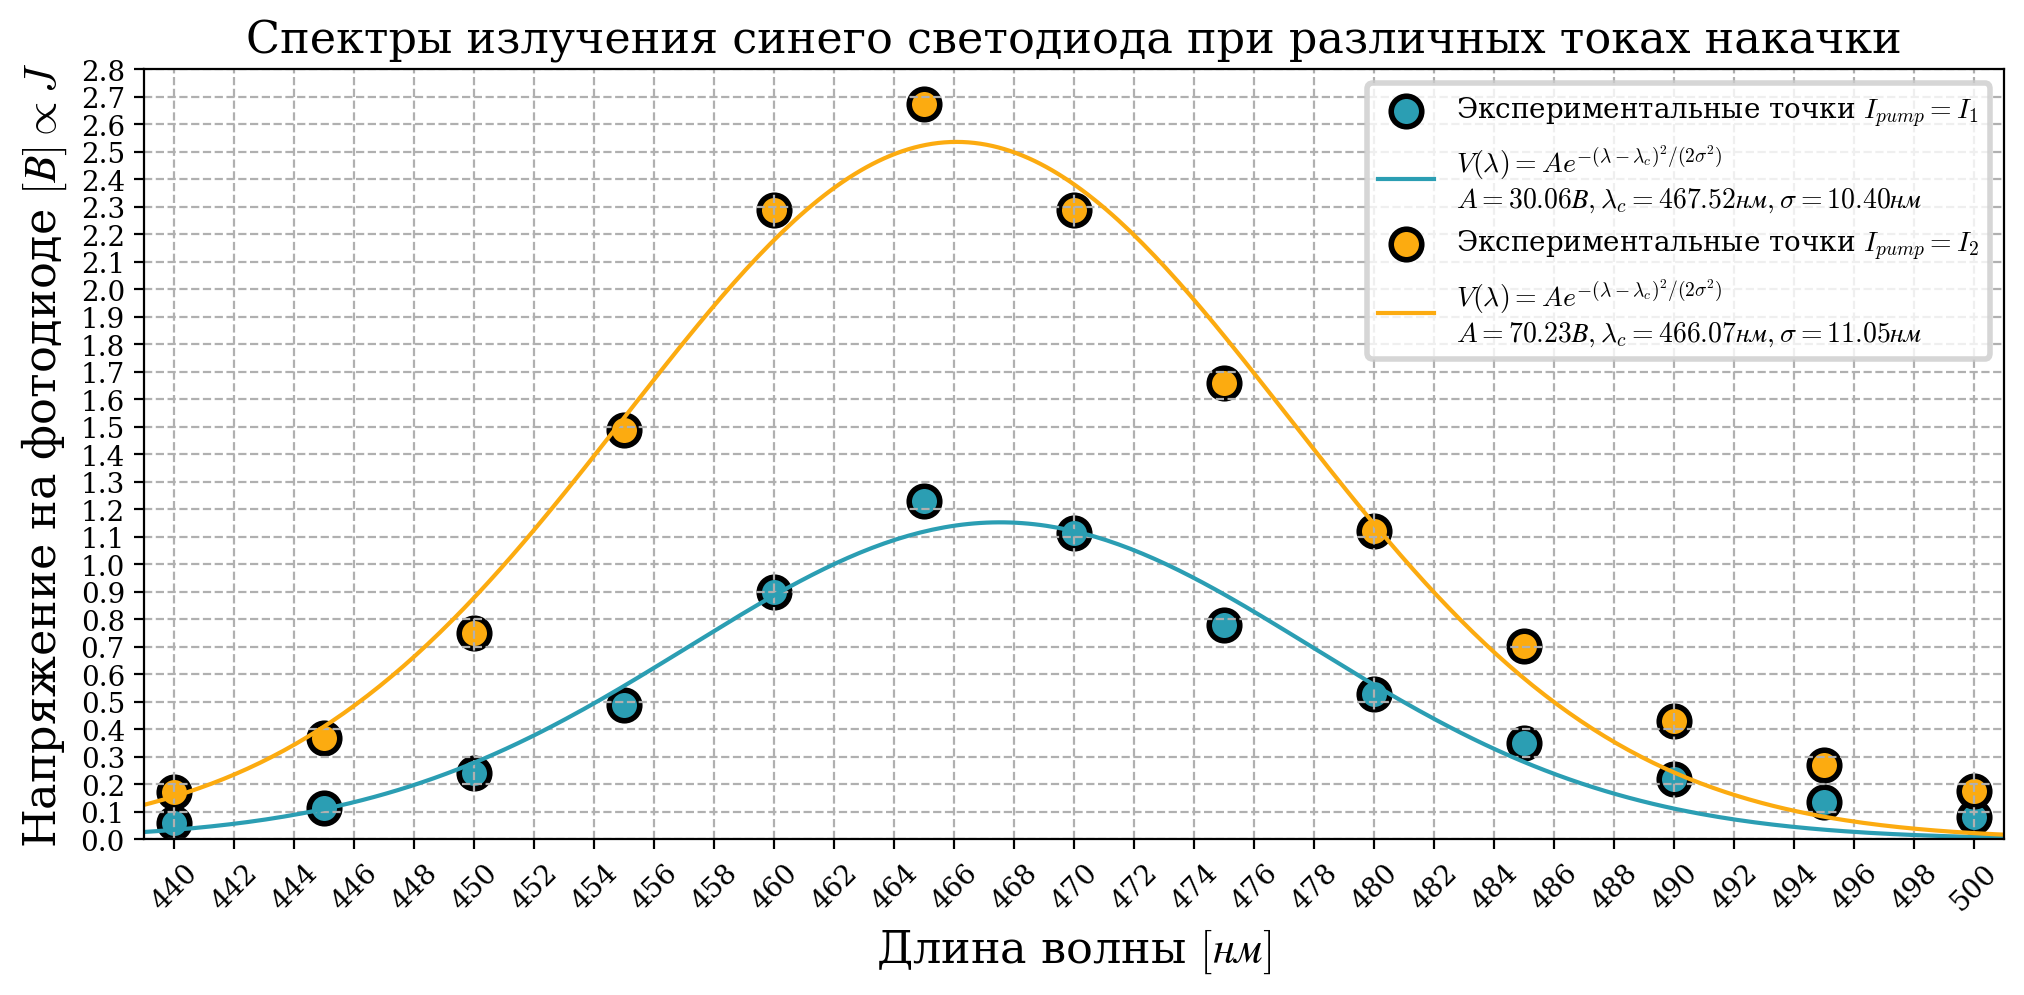
\includegraphics[width = 0.8\textwidth]{blue_gauss.png}
    \caption{Спектры излучения синего светодиода при различных токах накачки. Аппроксимация экспериментальных спектров кривой Гаусса.}
    \label{fig:blue_gauss}
\end{figure}


Экспериментальные кривые могут быть приближены Гауссианом. Результат аппроксимации экспериментальных данных  Гауссианом изображен на рисунке \ref{fig:blue_gauss}. Среднеквадратичная ошибка аппроксимации экспериментальных данных Гауссианом оказалась равной $MSE_{gauss} \sim 0.05$. 


\begin{figure}[htbp]
    \centering
    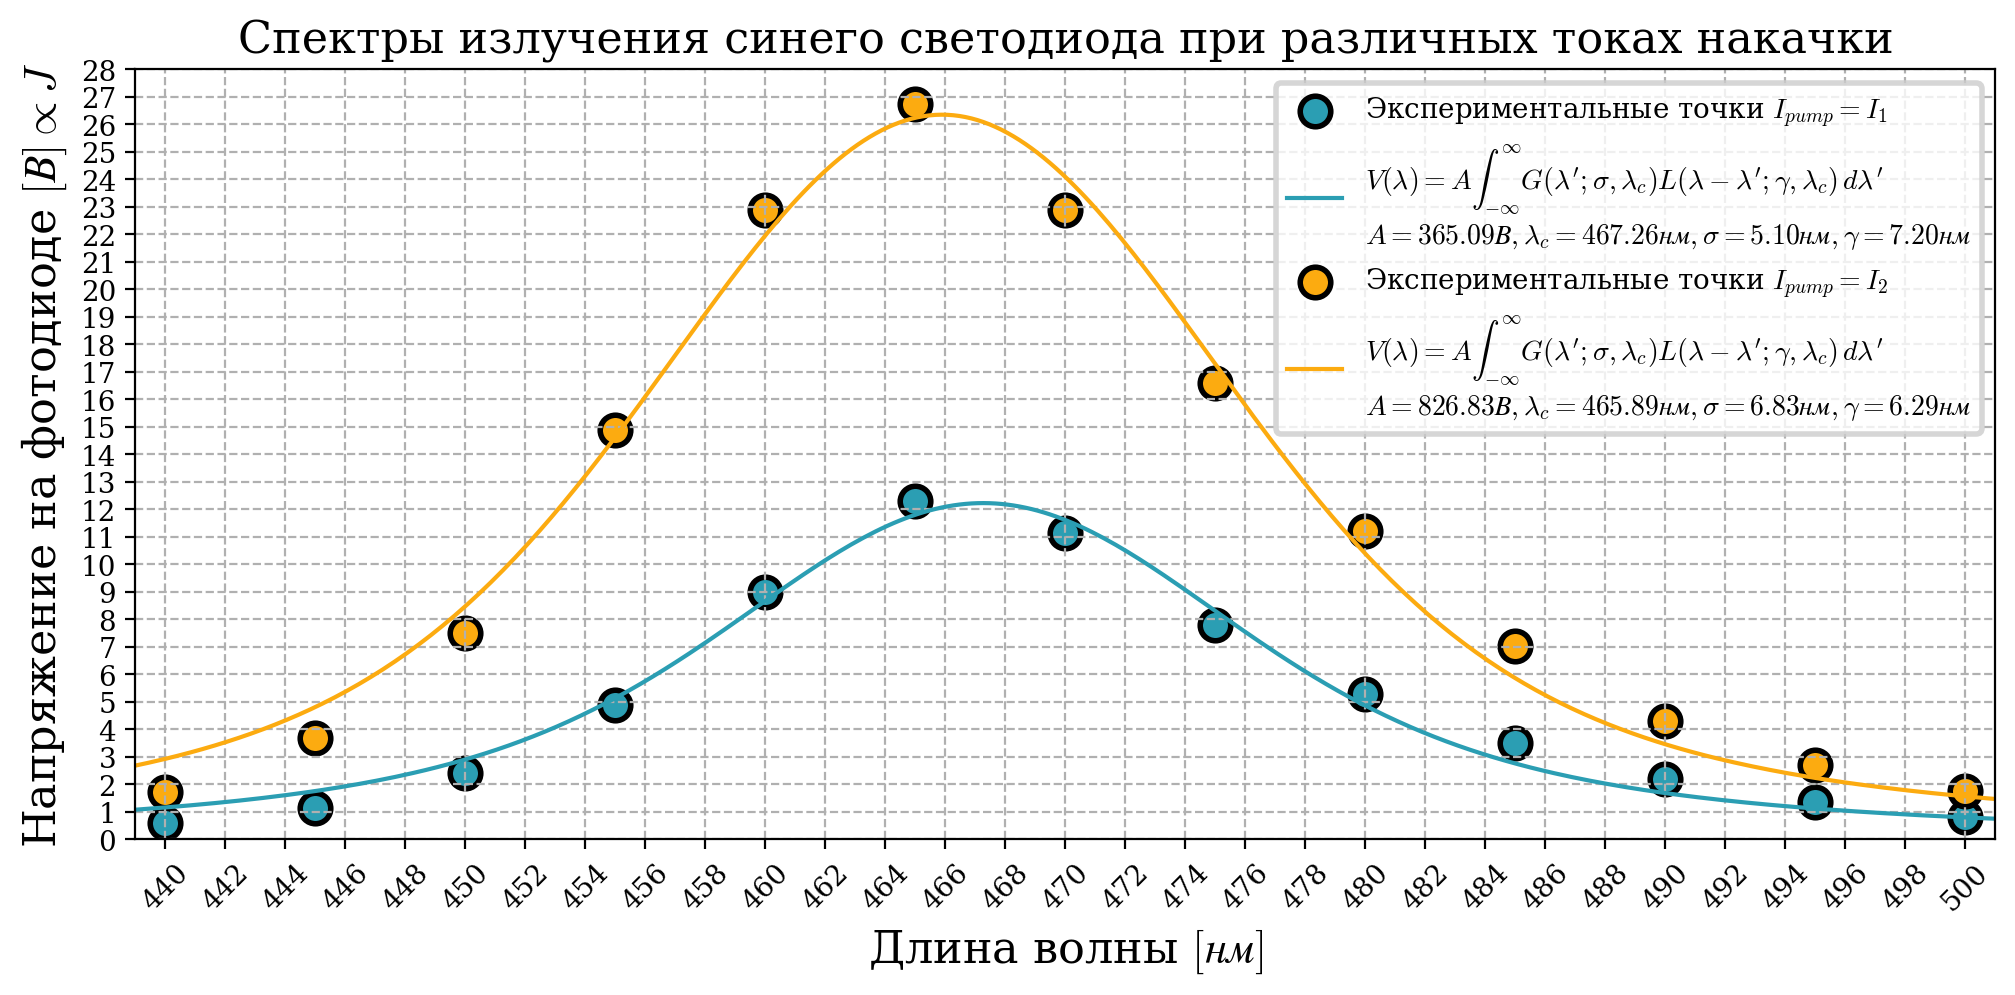
\includegraphics[width = 0.85\textwidth]{blue.png}
    \caption{Спектры излучения синего светодиода при различных токах накачки. Аппроксимация экспериментальных спектров кривой Фойгта.}
    \label{fig:blue}
\end{figure}


Для повышения точности следует использовать более сложную математическую модель. Известно два механизма уширения спектральных линий:
\begin{itemize}
    \item Гауссово уширение (доплеровское уширение) – вызвано движением частиц относительно наблюдателя (эффект Доплера). 
    \item Лоренцовское уширение (естественное уширение) – обусловлено квантовыми эффектами (конечное время жизни возбужденных состояний).
\end{itemize}

Дабы учесть оба механизма уширения спектра, удобно использовать контур Фойгта -- свертку контура Лоренца и Гаусса(смотрите формулу \ref{eq:voigt}).

\begin{equation}
    V(\lambda) = A \int_{-\infty}^{\infty} G(\lambda'; \sigma, \lambda_c) L(\lambda - \lambda'; \gamma, \lambda_c) \, d\lambda'
    \label{eq:voigt}
\end{equation}
\begin{itemize}
    \item $A$ - нормировочный параметр
    \item $G(\lambda, \sigma, \lambda_c)$ - функция распределения Гаусса с математическим ожиданием $\lambda_c$ и дисперсией $\sigma$.
    \item $L(\lambda, \gamma, \lambda_c)$ - функция распределения Коши(контур Лоренца) с максимум $\lambda_c$ и шириной $\gamma$
\end{itemize}

Результаты приближения спектра контуром Фойгта изображены на рисунке \ref{fig:blue}. Среднеквадратичная ошибка приближения $MSE_{voigt} \sim 0.02$. Таким образом точность аппроксимации экспериментальных данных контуром Фойгта в два раза выше точности полученной при использовании контура Гаусса. Параметры оптимального контура $\gamma$ и $\sigma$ оказались равными по порядку -- то есть оба механизма уширения оказывают примерно одинаковое влияние на наблюдаемый спектр.



\subsection*{\textcolor{sub_header}{Спектральные характеристики излучения красного светодиода}}
\begin{figure}[htbp]
    \centering
    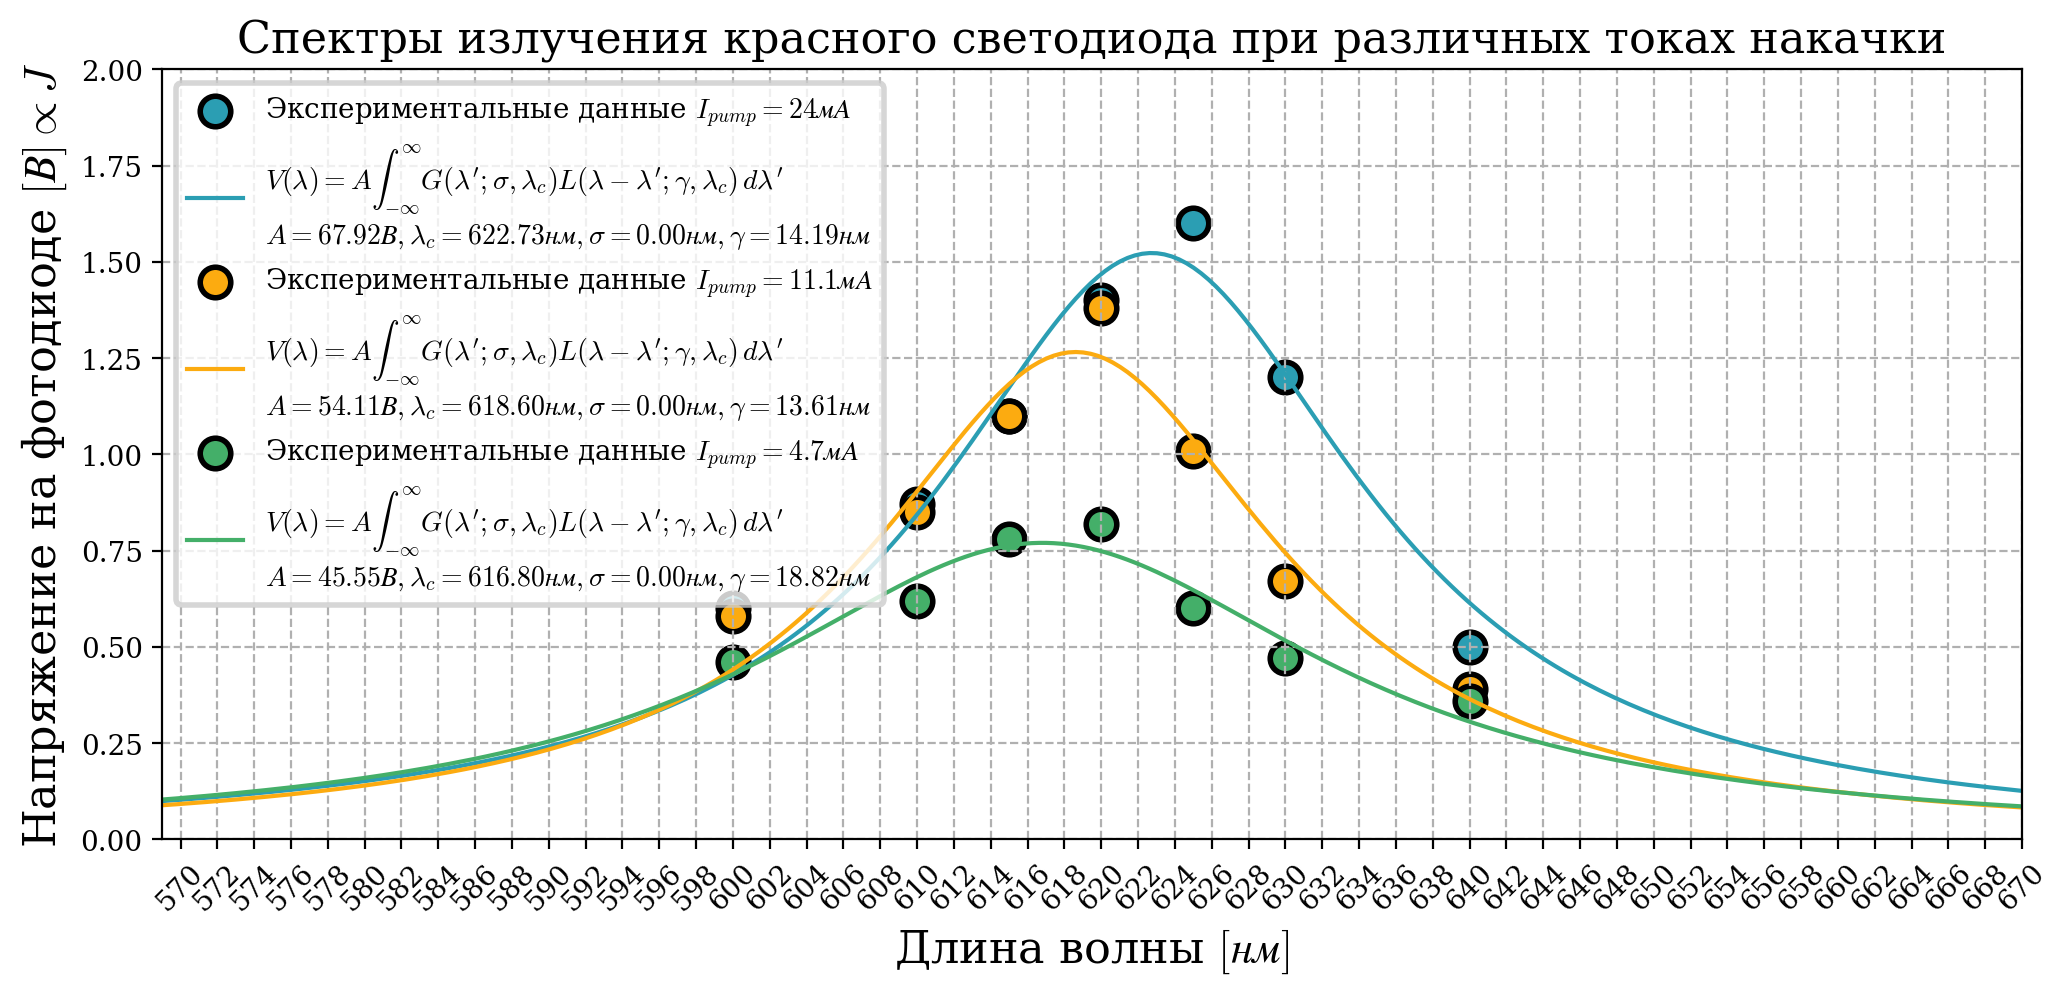
\includegraphics[width = 0.7\textwidth]{red.png}
    \caption{Спектры излучения красного светодиода при различных токах накачки}
    \label{fig:red}
\end{figure}

Аппроксимируем спектры излучения красного диода по формуле \ref{eq:voigt}. Значение $\gamma$ сильно превысило значение $\sigma$. Однако точность аппроксимации оказалась достаточно низкой, поэтому никаких выводов о природе уширения линии излучения красного светодиода сделать нельзя.

\subsection*{\textcolor{sub_header}{Спектральные характеристики излучения зеленого светодиода}}

\begin{figure}[htbp]
    \centering
    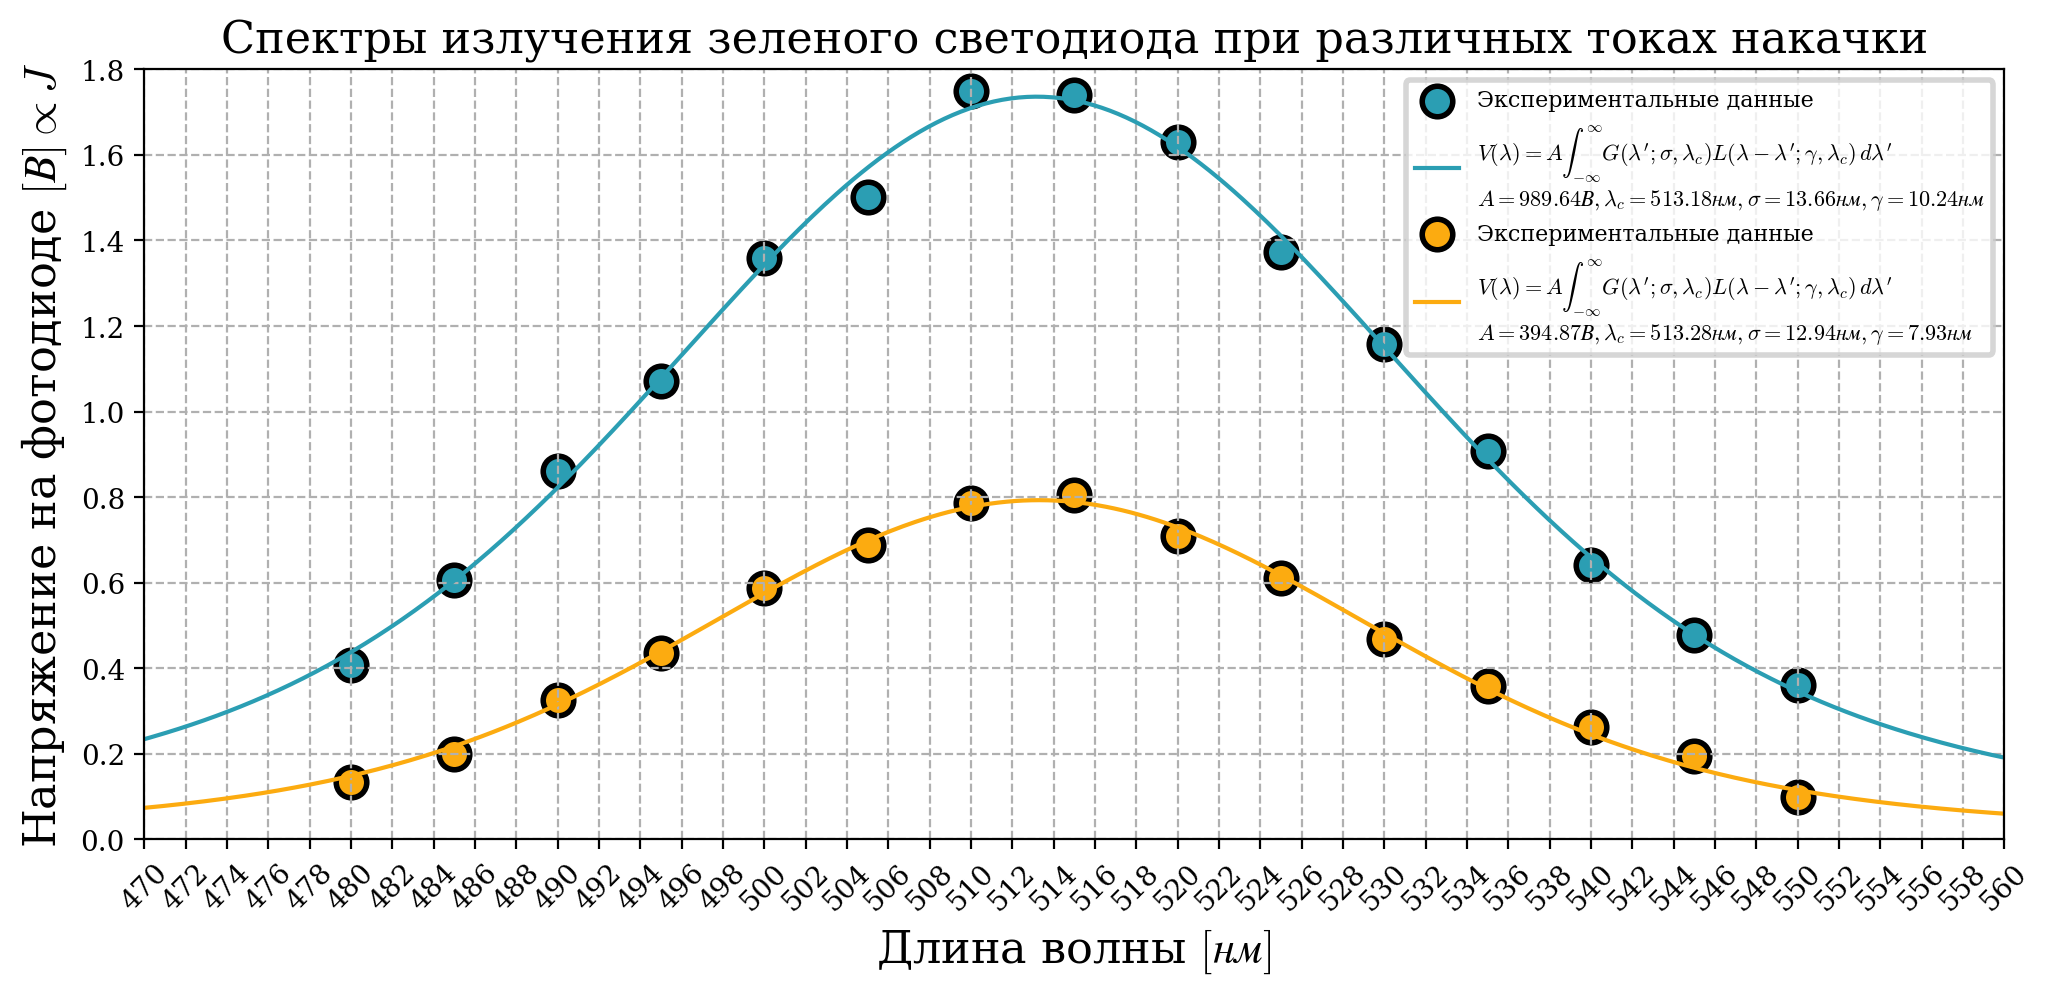
\includegraphics[width = 0.8\textwidth]{green.png}
    \caption{Спектры излучения зеленого светодиода при различных токах накачки}
    \label{fig:green}
\end{figure}

Результат аппроксимации экспериментально полученных спектров излучения зеленого светодиода изображен на рисунке \ref{fig:green}. Оптимальные $\gamma$ и $\sigma$ вновь оказались равны по порядку, оба механизма уширения оказывают одинаковое влияние на спектры.


В таблице \ref{tab:sample} представлены результаты аппроксимации экспериментальных данных. 
\begin{table}[h!]
    \centering
    \begin{tabular}{|c|c|c|c|c|}
    \hline
    \textbf{Образец} & \textbf{$\lambda_c$} [нм] & \textbf{$\gamma$} [нм] & \textbf{$\sigma$} [нм] \\ \hline
    
    Синий светодиод, маленький ток накачки & 467  & 7.2 & 5.1 \\ \hline
    Синий светодиод, большой ток накачки &  466 & 6.2 & 6.8 \\ \hline
    Красный светодиод, $J_{\text{накачки}} = 24$мА & 623 & 14.2 & 0\\ \hline
    Красный светодиод, $J_{\text{накачки}} = 11.1$мА & 620 & 13.6 & 0 \\ \hline
    Красный светодиод, $J_{\text{накачки}} = 4.7$мА & 616 & 18.8 & 0 \\ \hline
    Зеленый светодиод, большой ток накачки & 513.2 & 10.2 & 13.7 \\ \hline
    Зеленый светодиод, маленький ток накачки & 513.2 & 7.9 & 13 \\ \hline

    \end{tabular}
    \caption{Результаты аппроксимации экспериментально полученных спектров.}
    \label{tab:sample}
\end{table}
    



\section*{\textcolor{header}{Вывод}}

\begin{itemize}
    \item Удалось снять входную характеристику красного светодиода. Аппроксимируя экспериментальные данные формулой \ref{eq:vc} удалось оценить мощность накачки при которой светодиод входит в насыщение. Она оказалась равной $P_{\text{насыщения}} \sim 175$мВт.
    \item Удалось найти пороговую мощность генерации полупроводникового лазера. $P_{\text{пороговая}} \sim 40 мВт$.
    \item Уширение линии излучения светодиода связано как с Доплеровским механизмом так и с Лоренцевским. Максимальная точность аппроксимации экспериментальных данных достигается при учете обоих механизмов.
    \item Увеличение мощности накачки приводит к уширению спектра, а также к небольшому увеличению длины волны генерации. Большая мощность накачки влечет рост средней скорости носителей, спектр становится шире за счет Доплеровского механизма.
    \item Точность аппроксимации спектра красного светодиода значительно ниже точности аппроксимации прочих данных. Низкая точность может быть связана с малым количеством точек. 
    \item Для повышения точности эксперимента следует учитывать спектральные характеристики используемого фотоприёмника.
\end{itemize}



\section*{\textcolor{header}{P.S.}}
В ходе своего обучения в бакалавриате мне довелось написать множество отчетов. Этот отчет — последний. Мне всегда приносили удовольствие лабораторные работы: процесс сбора данных, их последующая обработка. Огромная благодарность всем преподавателям, которые вели у меня лабораторный практикум — с вами было интересно и увлекательно!




\section*{\textcolor{header}{Приложение}}

\begin{table}[h]
    \centering
    
    \begin{tabular}{|c|c|c|}
        \hline
        Upump, V & Ipump, mA & Iph, \textmu A \\
        \hline
        3.69 & 1.79 & 2 \\
        4.02 & 3.19 & 4 \\
        4.28 & 4.24 & 8 \\
        4.51 & 5.75 & 8 \\
        4.68 & 6.96 & 12 \\
        4.87 & 9.13 & 18 \\
        5.09 & 10.8 & 20 \\
        5.46 & 17.9 & 23 \\
        5.52 & 19.9 & 26 \\
        5.83 & 31.8 & 33 \\
        \hline
    \end{tabular}
    \caption{Выходная характеристика красного светодиода}
\end{table}

\begin{table}[h]
    \centering
    
    \begin{tabular}{|c|c|c|c|}
        \hline
        Upump, V & Ipump, mA & Ppump, mW & Iph, \textmu A \\
        \hline
        2.73 & 17.35 & 47.3655 & 150 \\
        2.74 & 17.58 & 48.1692 & 185 \\
        2.74 & 17.8 & 48.772 & 213 \\
        2.75 & 17.94 & 49.335 & 258 \\
        2.71 & 16.08 & 43.5768 & 36 \\
        2.68 & 15.9 & 42.612 & 6 \\
        \hline
    \end{tabular}
    \caption{Выходная характеристика ПИЛ}
\end{table}

\begin{table}[h]
    \centering
    
    \begin{tabular}{|c|c|c|}
        \hline
        $\lambda$, нм & $U$, В & $U$, В \\
        \hline
        440 & 0.59 & 1.74 \\
        445 & 1.15 & 3.68 \\
        450 & 2.40 & 7.50 \\
        455 & 4.90 & 14.9 \\
        460 & 9.00 & 22.9 \\
        465 & 13.20 & 26.75 \\
        470 & 11.15 & 22.9 \\
        475 & 7.80 & 16.6 \\
        480 & 5.30 & 11.2 \\
        485 & 3.50 & 7.05 \\
        490 & 2.20 & 4.32 \\
        495 & 1.35 & 2.70 \\
        500 & 0.83 & 1.77 \\
        \hline
    \end{tabular}
    \caption{Спектры синего светодиода при различных токах накачки}
\end{table}

\begin{table}[h]
    \centering
    
    \begin{tabular}{|c|c|c|}
        \hline
        $\lambda$, нм & $U$, В & $U$, В \\
        \hline
        480 & 4.07 & 1.35 \\
        485 & 6.06 & 2.00 \\
        490 & 8.62 & 3.25 \\
        495 & 10.71 & 4.36 \\
        500 & 13.0 & 5.87 \\
        505 & 15.02 & 6.89 \\
        510 & 17.50 & 7.87 \\
        515 & 17.40 & 8.05 \\
        520 & 16.30 & 7.10 \\
        525 & 13.74 & 6.10 \\
        530 & 11.57 & 4.68 \\
        535 & 9.07 & 3.58 \\
        540 & 6.42 & 2.62 \\
        545 & 4.78 & 1.95 \\
        550 & 3.61 & 1.00 \\
        \hline
    \end{tabular}
    \caption{Спектры зелёного светодиода при различных токах накачки}
\end{table}

\begin{table}[h]
    \centering
    
    \begin{tabular}{|c|c|c|c|}
        \hline
        $\lambda$, нм & $U$, В (24mA) & $U$, В (11.1mA) & $U$, В (4.7mA) \\
        \hline
        570 & 0.36 & 0.35 & 0.35 \\
        590 & 0.46 & 0.44 & 0.39 \\
        600 & 0.60 & 0.58 & 0.46 \\
        610 & 0.87 & 0.85 & 0.62 \\
        615 & 1.1 & 1.1 & 0.78 \\
        620 & 1.4 & 1.38 & 0.82 \\
        625 & 1.6 & 1.1 & 0.87 \\
        630 & 1.2 & 0.67 & 0.47 \\
        650 & 0.38 & 0.35 & 0.36 \\
        640 & 0.50 & 0.39 & 0.36 \\
        \hline
    \end{tabular}
    \caption{Спектры красного светодиода при различных токах накачки}
\end{table}

\end{document}
